%; whizzy section -pdf xpdf -latex ./whizzypdfptex.sh
% latex beamer presentation.
% platex, latex-beamer でコンパイルすることを想定。 

%     Tokyo Debian Meeting resources
%     Copyright (C) 2008 Junichi Uekawa

%     This program is free software; you can redistribute it and/or modify
%     it under the terms of the GNU General Public License as published by
%     the Free Software Foundation; either version 2 of the License, or
%     (at your option) any later version.

%     This program is distributed in the hope that it will be useful,
%     but WITHOUT ANY WARRANTY; without even the implied warranty of
%     MERCHANTABILITY or FITNESS FOR A PARTICULAR PURPOSE.  See the
%     GNU General Public License for more details.

%     You should have received a copy of the GNU General Public License
%     along with this program; if not, write to the Free Software
%     Foundation, Inc., 51 Franklin St, Fifth Floor, Boston, MA  02110-1301 USA

\documentclass[cjk,dvipdfmx,12pt]{beamer}
\usetheme{Tokyo}
\usepackage{ulem}
\usepackage{tabularx}

\usepackage{fancybox}
\usepackage{fancyvrb}   
\usepackage{float}

% commandline環境を定義。画面入出力についてはcommandline環境
% で表記する
\newenvironment{commandline}%
{\VerbatimEnvironment
  \begin{Sbox}\begin{minipage}{0.9\hsize}\begin{fontsize}{7.3}{7.3} \begin{BVerbatim}}%
{\end{BVerbatim}\end{fontsize}\end{minipage}\end{Sbox}
  \setlength{\fboxsep}{8pt}
% start on a new paragraph

\vspace{6pt}% skip before
\fcolorbox{dancerdarkblue}{dancerlightblue}{\TheSbox}

\vspace{6pt}% skip after
}
%end of commandline

\definecolor{dancerdarkblue}{rgb}{0,0.08,0.45}
\definecolor{dancernormalblue}{rgb}{0.8,0.9,0.95}
\definecolor{dancerlightblue}{rgb}{0.8,0.95,1}


%  preview (shell-command (concat "evince " (replace-regexp-in-string "tex$" "pdf"(buffer-file-name)) "&"))
%  presentation (shell-command (concat "xpdf -fullscreen " (replace-regexp-in-string "tex$" "pdf"(buffer-file-name)) "&"))

%http://www.naney.org/diki/dk/hyperref.html
%日本語EUC系環境の時
\AtBeginDvi{\special{pdf:tounicode EUC-UCS2}}
%シフトJIS系環境の時
%\AtBeginDvi{\special{pdf:tounicode 90ms-RKSJ-UCS2}}

\title{東京エリア Debian 勉強会}
\subtitle{資料}
\author{上川 純一 dancer@debian.org\\IRC nick: dancerj}
\date{2008年1月19日}
\logo{
\includegraphics[width=8cm]{image200607/openlogo-light.eps}}


% 間のタイトルページ用
\newcommand{\emtext}[1]{
\begin{frame}{}
 
\begin{minipage}{0.55\hsize}
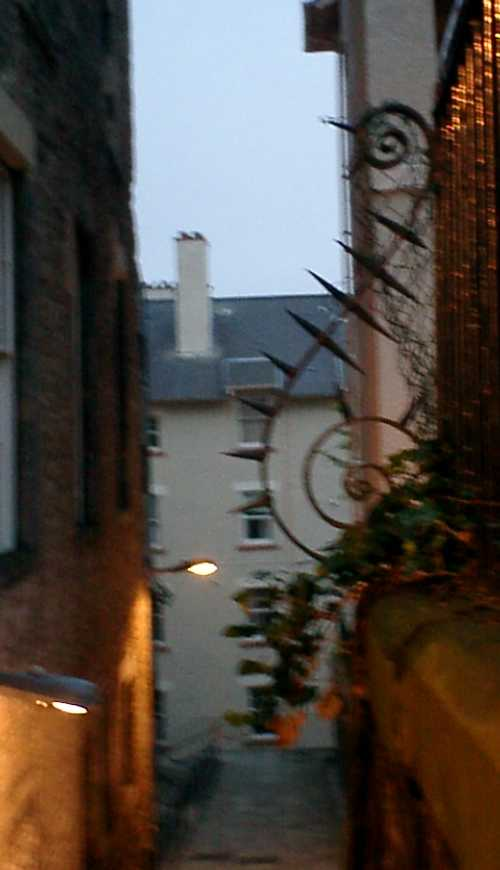
\includegraphics[width=1\hsize]{image200707/gurutitle.jpg}
\end{minipage}
\begin{minipage}{0.39\hsize}
 {\Huge #1
 }
\end{minipage}
\end{frame}
}

% 三択問題用
\newcounter{santakucounter}
\newcommand{\santaku}[5]{%
\addtocounter{santakucounter}{1}
\frame{\frametitle{問題\arabic{santakucounter}. #1}
%問題\arabic{santakucounter}. #1
\begin{minipage}[t]{0.8\hsize}
 \begin{itemize}
 \item
      \begin{minipage}{0.2\hsize}
      
\includegraphics[width=0.9\hsize]{image200703/janken-A.png}\end{minipage} 
       \begin{minipage}{0.6\hsize}
       A #2\end{minipage}\\
 \item
      \begin{minipage}{0.2\hsize}
      
\includegraphics[width=0.9\hsize]{image200703/janken-B.png}\end{minipage} 
       \begin{minipage}{0.6\hsize}
       B #3\end{minipage}\\
 \item
      \begin{minipage}{0.2\hsize}
      
\includegraphics[width=0.9\hsize]{image200703/janken-C.png}\end{minipage} 
       \begin{minipage}{0.6\hsize}
       C #4\end{minipage}\\
 \end{itemize}
\end{minipage}
}
\frame{\frametitle{問題\arabic{santakucounter}. #1}
%問題\arabic{santakucounter}. #1
\begin{minipage}[t]{0.8\hsize}
\begin{itemize}
 \item
      \begin{minipage}{0.2\hsize}
      
\includegraphics[width=0.9\hsize]{image200703/janken-A.png}\end{minipage} 
       \begin{minipage}{0.6\hsize}
       A #2\end{minipage}\\
 \item
      \begin{minipage}{0.2\hsize}
      
\includegraphics[width=0.9\hsize]{image200703/janken-B.png}\end{minipage} 
       \begin{minipage}{0.6\hsize}
       B #3\end{minipage}\\
 \item
      \begin{minipage}{0.2\hsize}
      
\includegraphics[width=0.9\hsize]{image200703/janken-C.png}\end{minipage} 
       \begin{minipage}{0.6\hsize}
       C #4\end{minipage}\\
\end{itemize}
\end{minipage}
\begin{minipage}[t]{0.15\hsize}
答えは:

\vspace{1cm}

  {\huge \hspace{1cm}#5}
  \hspace{-6cm}\includegraphics[width=4cm]{image200703/janken-#5.png}
 \end{minipage}}
}

\begin{document}

\frame{\titlepage{}}


\section{Intro}

\emtext{設営準備にご協力ください}

\begin{frame}
 \frametitle{Agenda}
\begin{minipage}[t]{0.45\hsize}
  \begin{itemize}
  \item 注意事項
	\begin{itemize}
	 \item 飲食禁止
	 \item 政治/宗教/営利活動禁止
	\end{itemize}
  \item quiz
  \item 最近のDebian関連のイベント
	\begin{itemize}
	 \item 前回
	\end{itemize}
 \end{itemize}
\end{minipage} 
\begin{minipage}[t]{0.45\hsize}
 \begin{itemize}
  \item 2008年度 Debian 勉強会企画
  \item Debian Package 管理の流れ
 \end{itemize}
\end{minipage}
\end{frame}

\section{最近}


\begin{frame}
 \frametitle{前回のアジェンダ}
\begin{minipage}[t]{0.45\hsize}
  \begin{itemize}
  \item 注意事項
	\begin{itemize}
	 \item 飲食禁止
	 \item 政治/宗教/営利活動禁止
	\end{itemize}
  \item quiz
  \item 最近のDebian関連のイベント
	\begin{itemize}
	 \item 前回
	\end{itemize}
 \end{itemize}
\end{minipage} 
\begin{minipage}[t]{0.45\hsize}
 \begin{itemize}
  \item Debian勉強会資料はいかにつくられているか
  \item 2007年度の勉強会をふりかえる
  \item 2008年度計画ワークショップ
 \end{itemize}
\end{minipage}
\end{frame}

\begin{frame}
 \frametitle{前々回のアジェンダ}
\begin{minipage}[t]{0.45\hsize}
  \begin{itemize}
  \item quiz
  \item 最近のDebian関連のイベント
	\begin{itemize}
	 \item 前回
	 \item OSC Tokyo/Fall
	 \item KOF
	 \item Biella 宴会
	\end{itemize}
 \end{itemize}
\end{minipage} 
\begin{minipage}[t]{0.45\hsize}
 \begin{itemize}
  \item bluetooth
  \item livehelper
  \item tomoyo kernel module
  \item KOF
  \item OSC Tokyo/Fall
  \item 今後の計画
 \end{itemize}
\end{minipage}
\end{frame}

\section{DWN quiz}
\begin{frame}{Debian 常識クイズ}

Debian の常識、もちろん知ってますよね?
知らないなんて恥ずかしくて、知らないとは言えないあんなことやこんなこと、
みんなで確認してみましょう。

今回の出題範囲は、\url{http://lists.debian.org/debian-devel-announce/} にある最近の
アナウンス文書です。

\end{frame}




\subsection{問題}

%問題をコピペ

 \santaku
 {Debian Miniconf 7が開催される、Linux Conf Au はいつ開始か}
 {1月28日}
 {1月29日}
 {1月19日}
 {A}

 \santaku
 {lintian.debian.org は全アーカイブに対して実行した lintian の実行結果を報告してくれているページだが、
 メンテナ単位のウェブページのURLが変更になった。どうかわったか?}
 {http://www.youtube.com/email.html}
 {http://people.ubuntu.com/~liw/lintian/gutsy-i386-main/reports/maintainer/email.html}
 {http://lintian.debian.org/reports/maintainer/email.html}
 {C}

 \santaku
 {dpkg のシンボルファイルで何が実現できるか?}
 {共有ライブラリなんてつかってられないので全部DLLにしてみた依存関係}
 {共有ライブラリはどんなバージョンでもよくなるような依存関係}
 {共有ライブラリのバージョン付きシンボルをベースにした依存関係}
 {C}

 \santaku
 {http://wiki.debian.org/HelpDebian/Start には何がかかれているか}
 {なぜDebianに貢献するべきか}
 {Debianはなぜ存在するのか}
 {GNUの存在意義}
 {A}

 \santaku
 {d-iでの翻訳作業の省力化のための工夫を Christian Perrierが実施した。
 それはメッセージを使われかたの優先度によって分割するものだったが、何分割にしたか}
 {5}
 {4}
 {3}
 {A}

 \santaku
 {Fonts task force (http://wiki.debian.org/Fonts)は週次で何を確認するス
 クリプトを用意したか?}
 {Debianパッケージとしてはたしてどれだけのフォントファイルが存在するのか
 を棚卸する}
 {いかがわしい形のフォントを検出する}
 {うまく表示できないフォントを検出する}
 {A}

 \santaku
 {Lennyリリースに標準として含まれる予定のKDEはどれか}
 {KDE3.0}
 {KDE4.0}
 {KDE5.0}
 {A}

 \santaku
 {Debian-i18n meeting で {main,contrib,non-free}/i18n/Translation-* に対
 して何がおきたか}
 {Grisuが悟りを開いた}
 {AUTOBYHANDの仕組みを利用するようになった}
 {あきらめて変更しないことにした}
 {B}

 \santaku
 {FOSS.inの開催期間中にDDになったインド人は何人目のインド人DDか?}
 {1}
 {2}
 {4}
 {C}

 \santaku
 {insservでは何が実現できるか?}
 {自動でデータベースにinsert してくれる}
 {依存関係からinitスクリプトの実行順序を計算して実行}
 {ネームサービスの提供}
 {B}


\section{最近の話題}

\section{事前課題紹介}
\emtext{事前課題の紹介}
% pre work home work

\begin{frame}{事前課題問題}


\begin{enumerate}
 \item 「こんなDebianパッケージを作成してみました・作成してみようとして
       みたらここまでしかできませんでした」\\
       2008年のDebian勉強会はDebianパッケージ作成について連続して企画を
       する予定です。現在どれくらいできるものなのか、どこらへんでつまっ
       ているのかを教えてください。(200-800文字)

 \item 「2008年のDebianの目玉を大胆に予想する」\\ 2008 年にどういう事が
       Debianの目玉になるのか、大胆に予想してみてください。
       (200-800文字)
\end{enumerate}

\end{frame}

% (query-replace "\\subsection" "\\end{frame}\\begin{frame}")
% (query-replace "\\subsubsection" "\\textbf")


\begin{frame}{吉田}

\textbf{「こんなDebianパッケージを作成してみました・作成してみようとしてみたらこ
こまでしかできませんでした」}
私は、たまに必要があると野良パッケージを作っています。
野良パッケージを作る理由としては、
\begin{enumerate}
 \item 	 使いたいアプリ/機能が公式パッケージにないから
 \item	 複数マシンにインストールしたり、環境再構築時に楽だから
 \item	 新規パッケージはstatbleに入らないから
 \item	 その他
\end{enumerate}
といったところです。
基本的には私のレベルは dh\_make して s で作るだけのレベルです。
その程度ですが、某LUGで入門として話してみたことがあります。
deb作成はrpm作成と比べて作業や決まり事が多くて少し面倒とおもいます。
が、仕事で作っていたrpmに比べて、
まだdebを作り慣れていないせいも多いと思います。
\end{frame}\begin{frame}{吉田}

\textbf{「2008年のDebianの目玉を大胆に予想する」}
lennyリリース!というのは皆書きそうなので...
某社からDebianプリインストール機が出る...とか
あると面白いですね(笑)。

\end{frame}\begin{frame}{日比野}

\textbf{こんなDebianパッケージを作成してみました}

仕事でも趣味でも必要があれば自分でもパッケージングをやってます。
debianディレクトリのテンプレートは、perlならdh-make-perlを、そうでなければdh\_makeを使っています。
ビルドはdebuildでlintianでチェックしています。
perlモジュールのNet::SSH::Perlのパッケージングを仕事でやったときが一番大変でした。
(sshをperlで実装してあるため、大量の依存モジュールが)
Cのヘッダの型情報と動的ライブラリを使ってCの関数をSchemeの処理系であるgaucheから呼び出すc-wrapperライブラリとか、
Cのソースコードを解析してObjective Camlの抽象木にしてくれるcilライブラリとかを趣味でパッケージングしました。

\end{frame}\begin{frame}{日比野}

\textbf{小ネタ: 2008年のDebianの目玉を大胆に予想する}

experimentalにはもう有るようですが perl-5.10 あたりでしょうか。
ぜんぜん大胆じゃない。
pythonとperlが両方ともparrotの上に乗るとか。


\end{frame}\begin{frame}{山本}

\textbf{「こんなDebianパッケージを作成してみました・作成してみようとしてみたらこ
こまでしかできませんでした」}
タールボールから野良ビルドする時は、必ずパッケージにすることにしています。
ただ、パッケージを2つ以上に分割する方法は、見様見まねで、よくわかってい
ません。
あと、新しいポリシー (3.7.3) の変更点もいまいち理解できていないと思います。

\textbf{「2008年のDebianの目玉を大胆に予想する」}

lenny フリーズ!
リリースは再来年に持ち越し!


\end{frame}\begin{frame}{山根}

\textbf{「こんなDebianパッケージを作成してみました・作成してみようとしてみたらここまでしかできませんでした」}

\begin{itemize}
 
 \item  JD という 2ch ブラウザをパッケージに。パッケージとしてはあまりいじらなくても良い状態になっています。upstream が活発なのでそれに併せて更新予定です。
 \item  eclipse-nls-sdk は、upstream が音沙汰無いのでどうしたものか。分割方法を考えた方がいいのが課題。とりあえず lintian の warning だけ何とかします。そう言えば今思い出しましたが、Pleiades をパッケージ化できないかを upstream な人に KOF で尋ねられていたのでした。すっかり忘れてた。これも検討しないといかんですね。
 \item  ccspatch (linux-patch-tomoyo)、ccstools (tomoyo-ccstools) につい
	ては一段落しました。backports を作って、upstream に利用を明示す
	る必要がありそうです。
\end{itemize}
\end{frame}
\begin{frame}{山根}
\begin{itemize}
 \item  mirmon というパッケージを作って ITP しましたが、mentors でスポンサーしてあげるよといった DD がそれっきり音沙汰無いのでどうしたものかと思っています。delel@jp で聞くべきかも。
 \item  フォントパッケージを増やしています。ttf-vlgothic、ttf-konatu、
	ttf-kiloji が今まで accepted。次は ttf-togoshi-gothic、ttf-ume
	が手元では出来ているので、細かな所を upstream に確認ののち、ITP
	→upload 予定。確認出来ているフリーなフォントはどんどん追加予定です。
 \item  sylph-searcher をパッケージにしたいな、と思ったのですが、libsylph を作らないといけないのですね。library package は今のところ作って無いのでどうしたものか。
\end{itemize}

 すでにパッケージを upload した人は、lintian.debian.org で自分のパッケージの warning を確認してどんどん潰すべきですな


\end{frame}\begin{frame}{前田}


\textbf{「こんなDebianパッケージを作成してみました・作成してみようとしてみたらこ
こまでしかできませんでした」}

年末年始でようやく一部のサーバをEtch化し始めました。ついでに自宅環境で使っているスクリプトの配布には、Debianパッケージにしてみようか、と思ったわけですね。で、じゃあスクリプトだけをパッケージ化するのはどうやるのかと、調べようとする前に、scpで転送してしまい、やらずじまいでした…。orz
何かのついでに始めてみようというのは、ダメですね…。今度の日曜(今月のDebian勉強会の翌日)ちゃんと時間を割いてやります。

\textbf{「2008年のDebianの目玉を大胆に予想する」}

きっと誰かがWiiもDebianにして、Wii Balance BoardでAPTシェルを自由自在に操っているに違いない。w

\end{frame}\begin{frame}{岩松 信洋}


\textbf{こんなDebianパッケージを作成してみました
  作成してみようとしてみたらここまでしかできませんでした}

最近作ったDebianパッケージは
\begin{itemize}
 \item  Macbook のLEDを Ethernetのアクセスに合わせて点灯させるソフトウェア
 \item  u-boot 用のイメージを作成するソフトウェア
\end{itemize}
です。

両方ともDebianパッケージ化を行い、手元で使っています。
パッケージ化がむずかしいソフトウェアではないので、特にハマることは
ありませんでした。

なので、いじられるところは特にありません。

\end{frame}\begin{frame}[containsverbatim]{Noriaki Sato}

以前、Ruby on Rails で Oracle を使うために
ruby-oci8 を install しようとしたら deb package が無かったので、
package を作ってみようとした事がありました。
\url{http://www.debian.org/doc/manuals/maint-guide/index.ja.html#contents}
辺り(古い?)を斜め読みしながらやったのですが、
\begin{commandline}
 $ dpkg-buildpackage -r fakeroot
\end{commandline}
した所で、何故か /usr/local 配下に install されてしまいました。
その時は、普通に install したのと同じ結果になっただけなので、
まあいっか、とゆー事で終わりにしてしまったのですが、
良い機会なので少し調べてみました。

\end{frame}\begin{frame}[containsverbatim]{Noriaki Sato}

\begin{commandline}
 
 $ tar xvfz ruby-oci8-1.0.0.tar.gz
 $ cd ruby-oci8-1.0.0
 $ dh_make -e mail_address -f ruby-oci8-1.0.0.tar.gz
 $ dpkg-buildpackage -r fakeroot
 (snip)
 dh_installdirs
 # Add here commands to install the package into debian/tmp
 /usr/bin/make DESTDIR=/home/noriaki/tmp/deb/ruby-oci8-1.0.0/debian/tmp install
 make[1]: ディレクトリ `/home/noriaki/tmp/deb/ruby-oci8-1.0.0' に入ります
 ruby setup.rb install
 ---> lib
 mkdir -p /usr/local/lib/site_ruby/1.8/
 install oci8.rb /usr/local/lib/site_ruby/1.8/
 Permission denied - /usr/local/lib/site_ruby/1.8/oci8.rb
 Try 'ruby setup.rb --help' for detailed usage.
\end{commandline}
ということで、いまさら Makefile を眺めてみた所、
そもそも DESTDIR がなく、install 先が簡単に変更出来ない感じでした。
Makefile から呼び出している setup.rb という script を読んで、
Makefile を書き換えないとダメっぽいです。
今回は時間がなく、ここまでで断念しました。
そもそも、package の作り方はまだ良く分かっていない所が多いので、
今日、ばっちり勉強して帰って、再度 try したいと思います。

\end{frame}\begin{frame}{高橋 昭之}

「こんなDebianパッケージを作成してみました・作成してみようとしてみたらここまでしかできませんでした」

作ってみたパッケージはGNU helloです。debian/rulesファイルを雛形のまま編集せずにdebuildが通ったので実力は全くついていませんが、dh\_makeなどの基本的なパッケージ作成コマンドの使い方は概ね把握しました。
これからパッケージ作成で学びたいことは、debian/rulesファイルのスタイル・書き方についてとgpg署名です。

「2008年のDebianの目玉を大胆に予想する」
初心者なので、2007年の目玉がなんだったのかさえ知りません:-(

\end{frame}\begin{frame}{Aya Komuro}

「こんなDebianパッケージを作成してみました・作成してみようとしてみたらこ
こまでしかできませんでした」

Debianパッケージは作成した事が無いです。以前作ったもの自体をパッケージ化
したほうがいいか?と考えたときに即座に必要ないと判断したのでパッケージ化
するネタが無いです。こんなのを作りたいなぁと妄想だけはあるんですけどね。

\end{frame}\begin{frame}{橋本 徹}

こんなDebianパッケージを作成してみました

Debianパッケージになっているソフトウェアは数多くあるし、非公式の
パッケージを作っている人も多いので自分でパッケージングする必要に
迫られることは少ないのだが、今までパッケージングしてみた数少ない
例としては以下のものが挙げられる。

* gnubg

gnubgは公式パッケージになっているが、公式パッケージが全然更新され
ていなかった時期にCVS版をビルドしてパッケージングしたことはあった。
autoconfを使用したものだったのでインストール可能なレベルのパッケ
ージを作るのは比較的容易だった。

\end{frame}\begin{frame}{橋本 徹}

* gtkipmsg

IP Messengerクライアントとしては、xipmsgは公式パッケージとして存在
するが、GTK版クライアントのgtkipmsgのパッケージは存在しなかったので
パッケージングしてみた。これもautoconf対応だったのでインストール可能
なパッケージは比較的容易に作成できた。

autoconfモノは比較的容易にパッケージングできることがわかった。
が、autoconfを使っていないものについてはまだ経験がない。

\end{frame}\begin{frame}{森田尚}

{「こんなDebianパッケージを作成してみました・
作成してみようとしてみたらここまでしかできませんでした」}

作ったパッケージ:

仕事である編集業や、趣味である日曜プログラミングでの必要性や興味から、次
の野良パッケージを作って使っています。

\end{frame}\begin{frame}{森田尚}

\begin{description}
 \item[vfdata-otf-ptex]
  \url{http://psitau.at.infoseek.co.jp/otf.html}
  OTFは、OpenTypeフォントをpTeXで使うためのTeXマクロパッケージおよび
  フォントデータです。OTF版のヒラギノやモリサワをDebianで使いたかった
  ので作りました。

 \item[ideotype]
  \url{http://ideotype.sourceforge.net/}
  IdeoTypeは、商業出版の現場で編集制作を支援するためのツールです。
  XHTML形式の原稿を本(PDF)に変換します。
\end{description}

\end{frame}\begin{frame}{森田尚}

これからパッケージ化しようと考えているもの:

\begin{description}
\item[libxsl-ruby]
	   \url{https://rubyforge.org/projects/libxsl/}
  libxsltをRubyで使うためのライブラリです(1文字違いのlibxslt-ruby
  とは異なる)。Rubyの拡張ライブラリをDebianパッケージにする際の
  作法がよく分からず、まだ眺めている程度です。

\item[c-wrapper]
	   \url{http://homepage.mac.com/naoki.koguro/prog/c-wrapper/index-j.html}
  SchemeインタプリタGaucheから、C/Objective-Cで書かれたライブラリを
  利用できる仕組み(FFI)です。
\end{description}

\end{frame}\begin{frame}{森田尚}

知りたいこと:

  他のパッケージ形式との間での変換の仕方(例えばRubyGemsのGemから
  dpkg形式への変換や、dpkg形式からRPMやMacPortsへの変換など)。Gem
  の場合、ほぼ自動での変換が可能らしいことは分かったのですが、
  ruby-pkg-toolsの使い方が分からず挫折中です。

\end{frame}\begin{frame}{森田尚}

パッケージ化されてほしいその他のソフトウェア:

\begin{description}
 \item[rushcheck]        Ruby用のテスティングツール
 \item[rspec]            Ruby用のテスティングツール
 \item[cruisecontrol.rb] continuous integrationサーバ
 \item[pdumpfs-rsync]    rsync越しのpdumpfs
 \item[pdumpfs-clean]    pdumpfsによるバックアップデータの整理・削除
 \item[color-moccur.el, moccur-edit.el]
                   Emacsで複数バッファを一括して検索・編集
\end{description}
\end{frame}


\emtext{2008年計画}

\begin{frame}{2008年計画}

{\scriptsize
\begin{enumerate}
 \item 新年会「気合を入れる」
 \item Open Source Conference Tokyo (3/1)
 \item データだけのパッケージを作成してみる、
       ライセンスの考え方 (David)
 \item バイナリ一つのパッケージを作成してみる (吉田@板橋)\\
       バージョン管理ツールを使いDebianパッケージを管理する(git)\\
       アップストリームの扱い(svn/git/cvs)(岩松 信洋さん)
 \item バイナリの分けたパッケージの作成。(前田さん)\\
       バイナリの分け方の考え方、アップグレードなどの運用とか。
 \item パッケージ作成(dpatch/debhelperで作成するパッケージ)(小林儀匡さん)\\
       man の書き方(roff or docbook)(でんさん)
 \item パッケージ作成(kernel patch、kernel module)
       、Debconf発表練習
 \item Debconf アルゼンチン、共有ライブラリパッケージ作成

 \item Open Source Conference Tokyo/Fall、
       デーモン系のパッケージの作成、latex、 emacs-lisp、フォントパッケージ
 \item パッケージの cross-compile の方法、amd64 上で i386 のパッケージと
       か、OSC-Fall報告会、Debconf報告会
 \item 国際化 po-debconf / po化 / DDTP
 \item 忘年会
\end{enumerate}
}
\end{frame}

\emtext{Debianパッケージ作成}

\section{}
\begin{frame}
  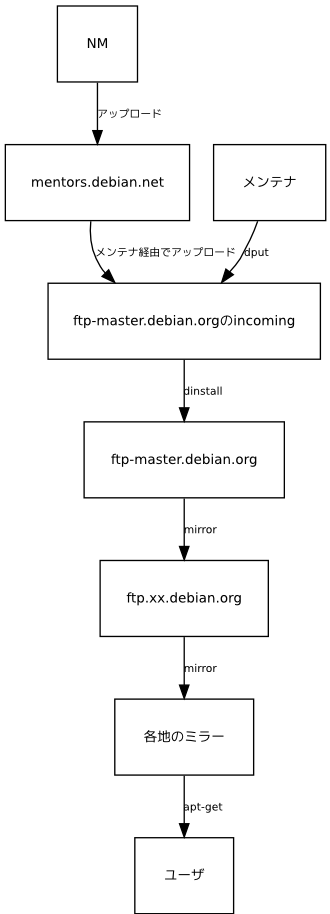
\includegraphics[height=1\vsize]{image200801/maint-package.png}
\end{frame}

\begin{frame}{開発者のロジックの流れ}
 \includegraphics[width=0.8\hsize]{image200801/devel-logic-i.eps}
\end{frame}

\emtext{アップストリーム取得}
\emtext{パッケージ作成}

\begin{frame}{BTSの対応}
\begin{itemize}
 \item  reportbug-ng 
 \item  reportbug
 \item  dpkg-dev-el 
\end{itemize}
\end{frame}

\begin{frame}[containsverbatim]{ChangeLog}
\begin{itemize}
 \item devscripts の dch
 \item dpkg-dev-el の debian-changelog.el
 \item vim の debchangelog 
\end{itemize}
\end{frame}

\begin{frame}{build-test}
\begin{itemize}
 \item debuild
 \item lintian / linda
 \item debc / debdiff
 \item debi
 \item pbuilder
\end{itemize}
\end{frame}

\emtext{アップロード}

\begin{frame}{レポジトリ作成}
 \begin{itemize}
  \item dpkg-scanpackages / dpkg-scansources 
  \item apt-ftparchive 
  \item mini-dinstall 
  \item apt-move 
  \item debarchiver
  \item reprepro
  \item dak
 \end{itemize}
\end{frame}

\section{}
\begin{frame}{宴会場所}

\begin{itemize}
 \item 宴会場所\\
       本日の宴会は「???」です。
  参加者は1Fに集合し、全員で移動しましょう。
 \item 片付け\\
       部屋を片付けるのにご協力ください。
\end{itemize}


\end{frame}

\end{document}

;;; Local Variables: ***
;;; outline-regexp: "\\([ 	]*\\\\\\(documentstyle\\|documentclass\\|emtext\\|section\\|begin{frame}\\)\\*?[ 	]*[[{]\\|[]+\\)" ***
;;; End: ***
